\section*{MASE}

\subsection*{SearcherLogo}
\begin{frame}
    \centering %Figura centrada.
    
\includegraphics[width=150px]{Assets/searcher_logo.png}
\end{frame}

\subsection*{Searcher}
    \begin{frame}
        \begin{abstract}
            En esta clase se procesa la consulta del usuario, retornando finalmente los resultados más acercados que se haya procesado.
        \end{abstract}
        \begin{figure}
            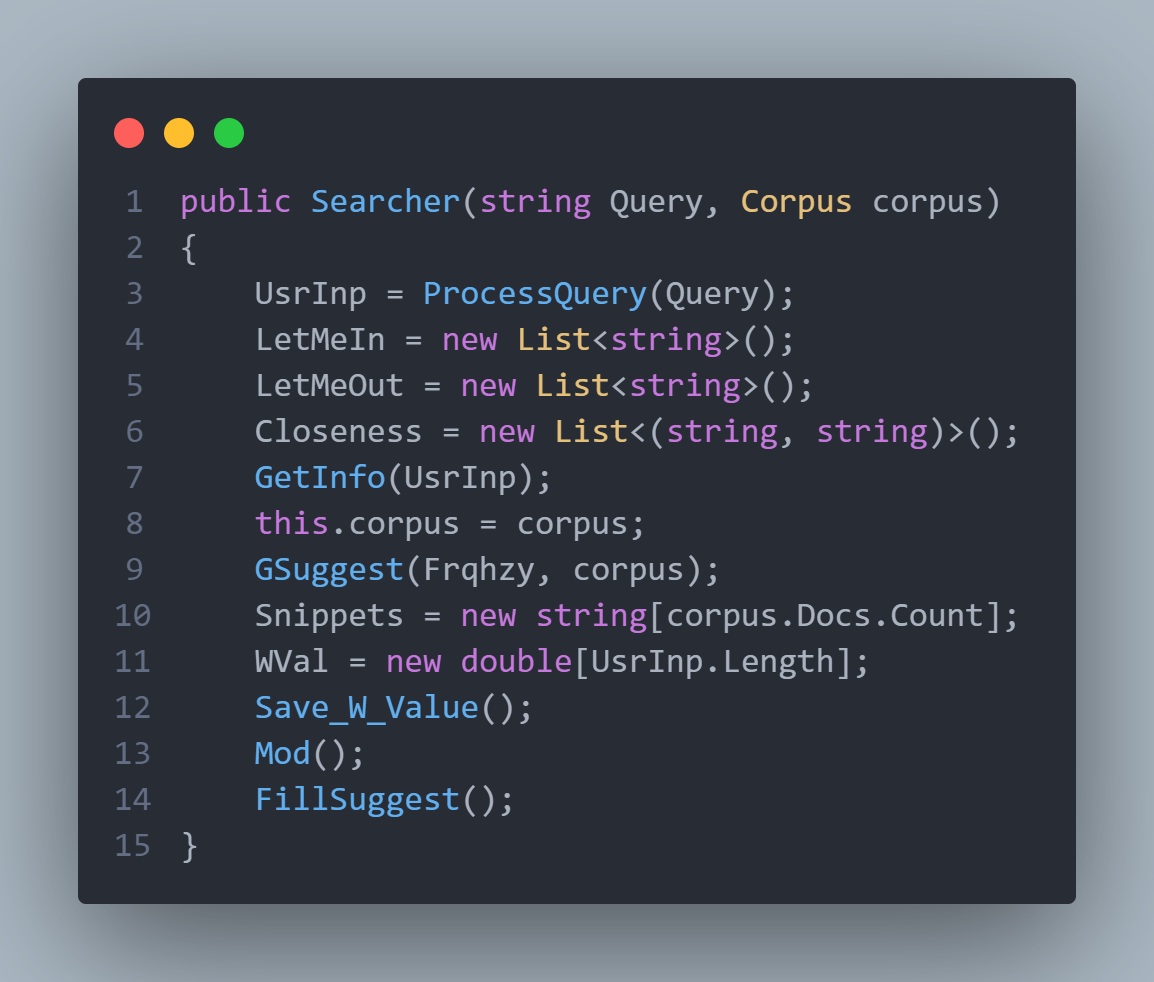
\includegraphics[width=200px]{Assets/searcher_builder.png}
        \end{figure}
    \end{frame}

    \begin{frame}
        En la anterior figura se pudieron observar unas cuantas funciones y elementos tales como:
        \begin{itemize}
            \item UsrInp, no es mas que la entrada del usuario separada por palabras.
            \item LetMeIn, LetMeOut, Closeness, son listas que se ejecutaran en dependencia de los operadores asignados
            \item GetInfo, GSuggest, Save\_W\_Value, Mod, FillSuggest, son funciones que estan explicadas en el Informe, en la sección MASE Searcher
            \item La linea que le otorga valor a "Snippets", será comentada más adelante, en la sección Snippet.
        \end{itemize}
        Igualmente haré un hincapié en la función GSuggest().
    \end{frame}

    \begin{frame}
        Esta función, se encargará de conseguir una sugerencia, de ahi GSuggest(GetSuggest), y para ello usará una función llamada Suggestion: 
        \begin{figure}
            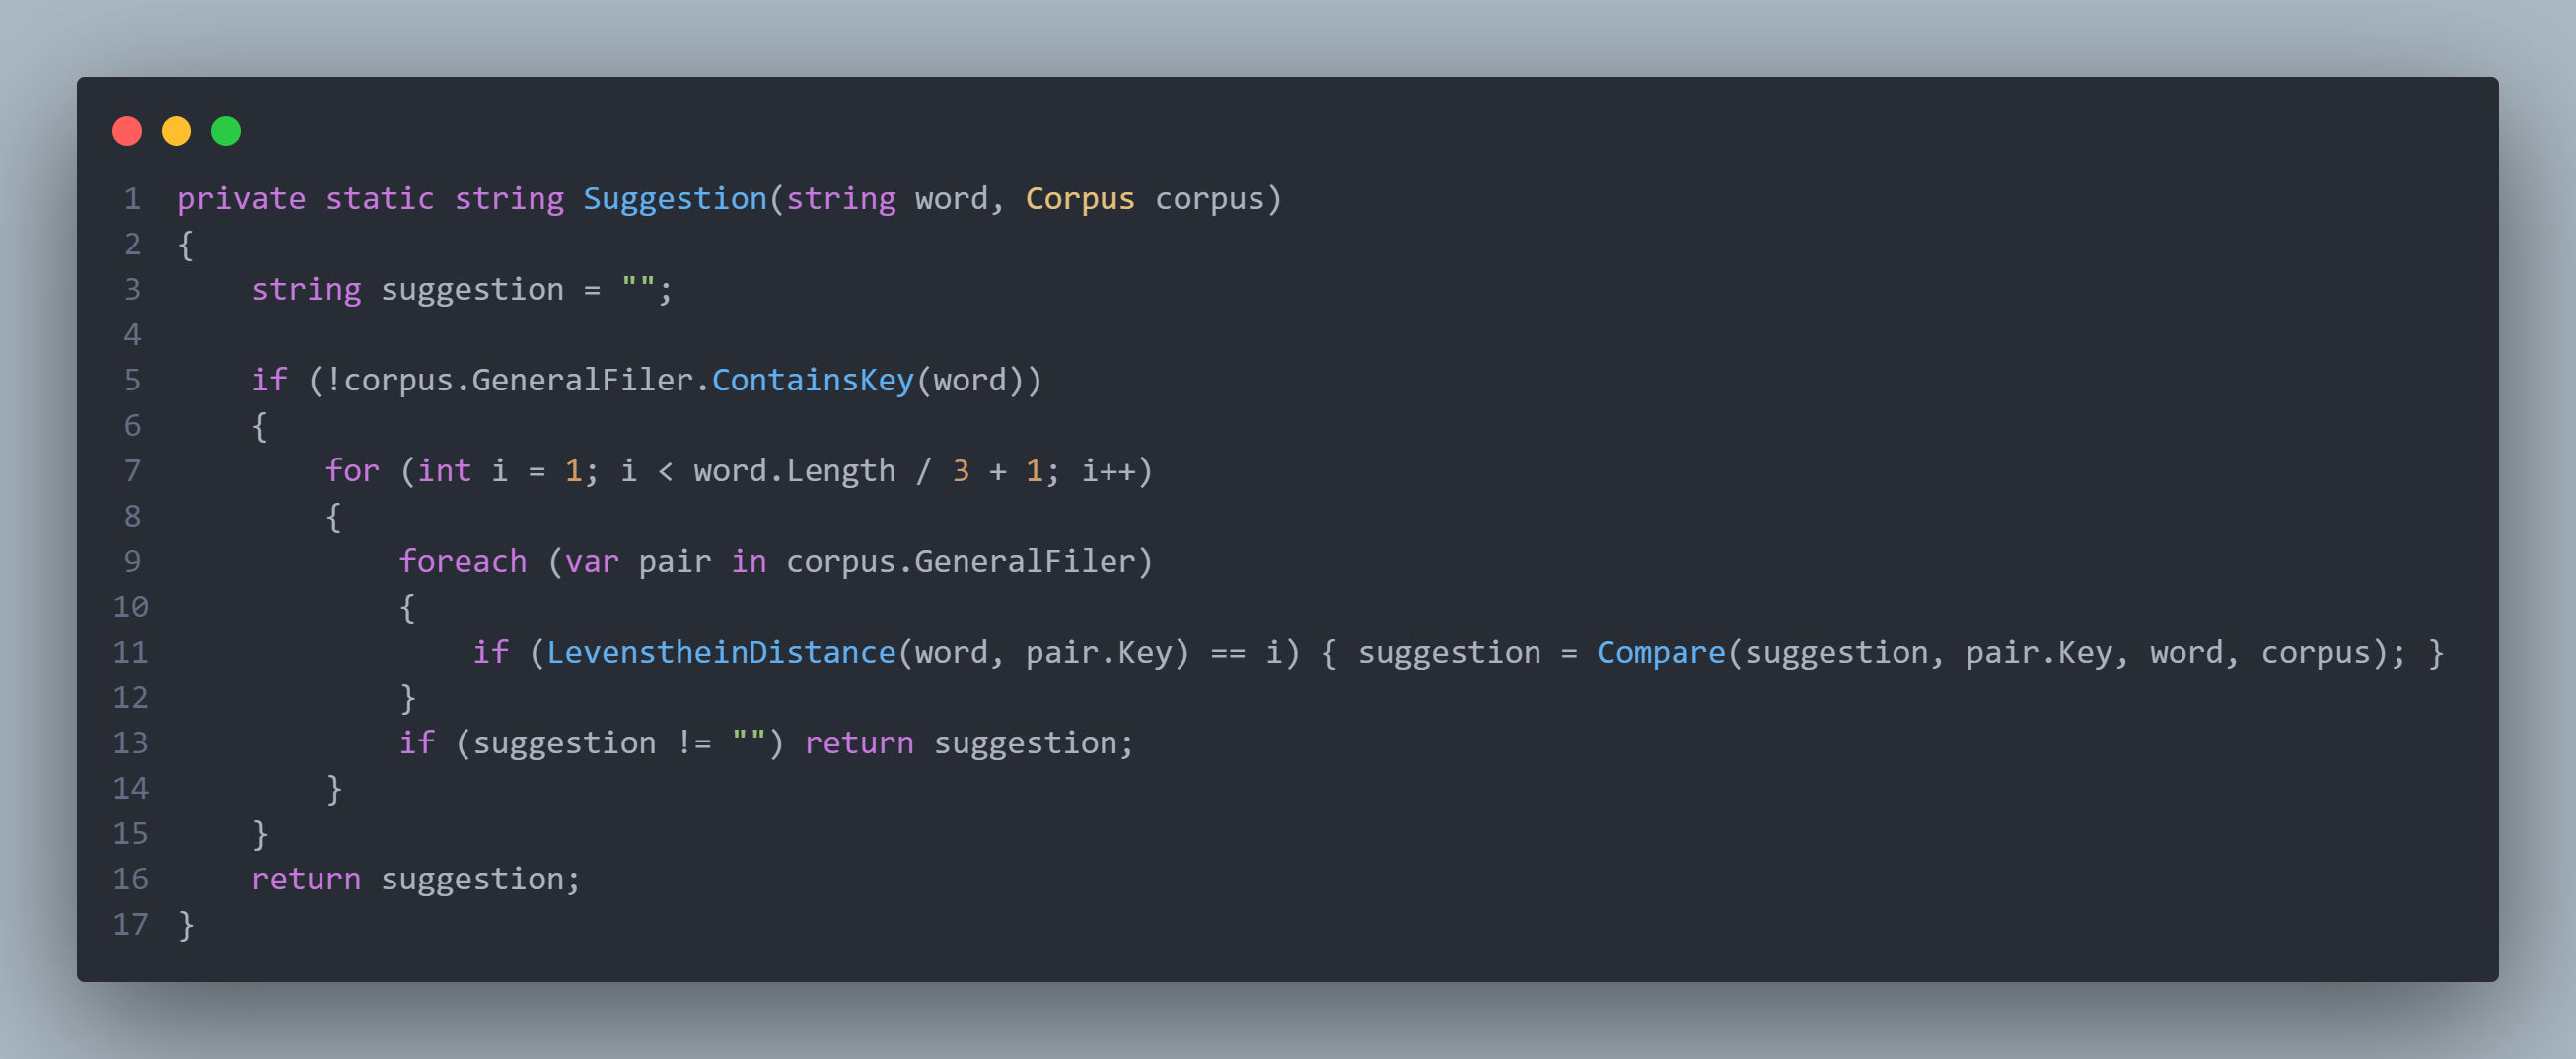
\includegraphics[width=220px]{Assets/suggestion.png}
        \end{figure}
        Esta función recorre el Vocabulario General(GeneralFiler), aplicando la distancia de Levensthein, par adevolver aquella palabra del VocabularioGeneral que se más similar a la consulta del usuario.
    \end{frame}

    
\subsection*{Score}
\begin{frame}
    \centering %Figura centrada.
    
\includegraphics[width=150px]{Assets/score_logo.png}
\end{frame}

\begin{frame}
    \begin{abstract}
        Esta clase tratará de obtener y colocar un puntaje adecuado a cada documento, que posteriormente sería mostrado.
        \begin{figure}
            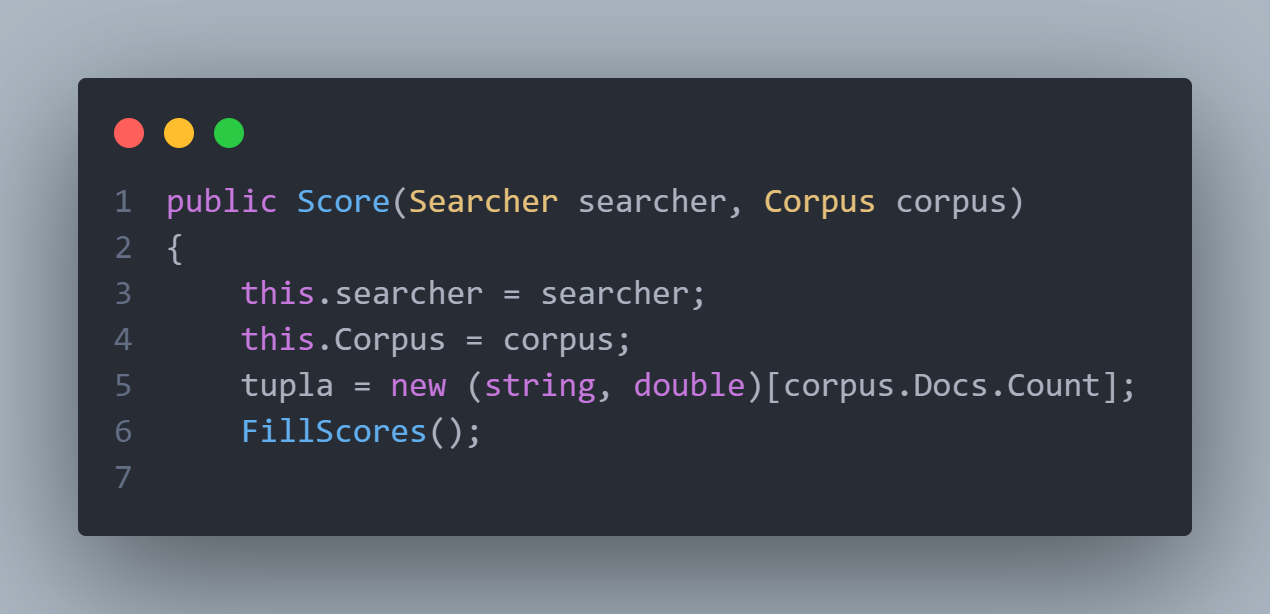
\includegraphics[width=200px]{Assets/score_builder.png}
        \end{figure}
        Previamente se habría creado una instacia de Searcher y de Corpus, aquí se toman. Además se crea una tupla de longitud = cantidad de documentos y la función FillScores() las ordenará de mayor a menor.
    \end{abstract}
\end{frame}

\begin{frame}
    Usará también además un producto vectorial comom se ve aquí a continuación.
    \begin{figure}
        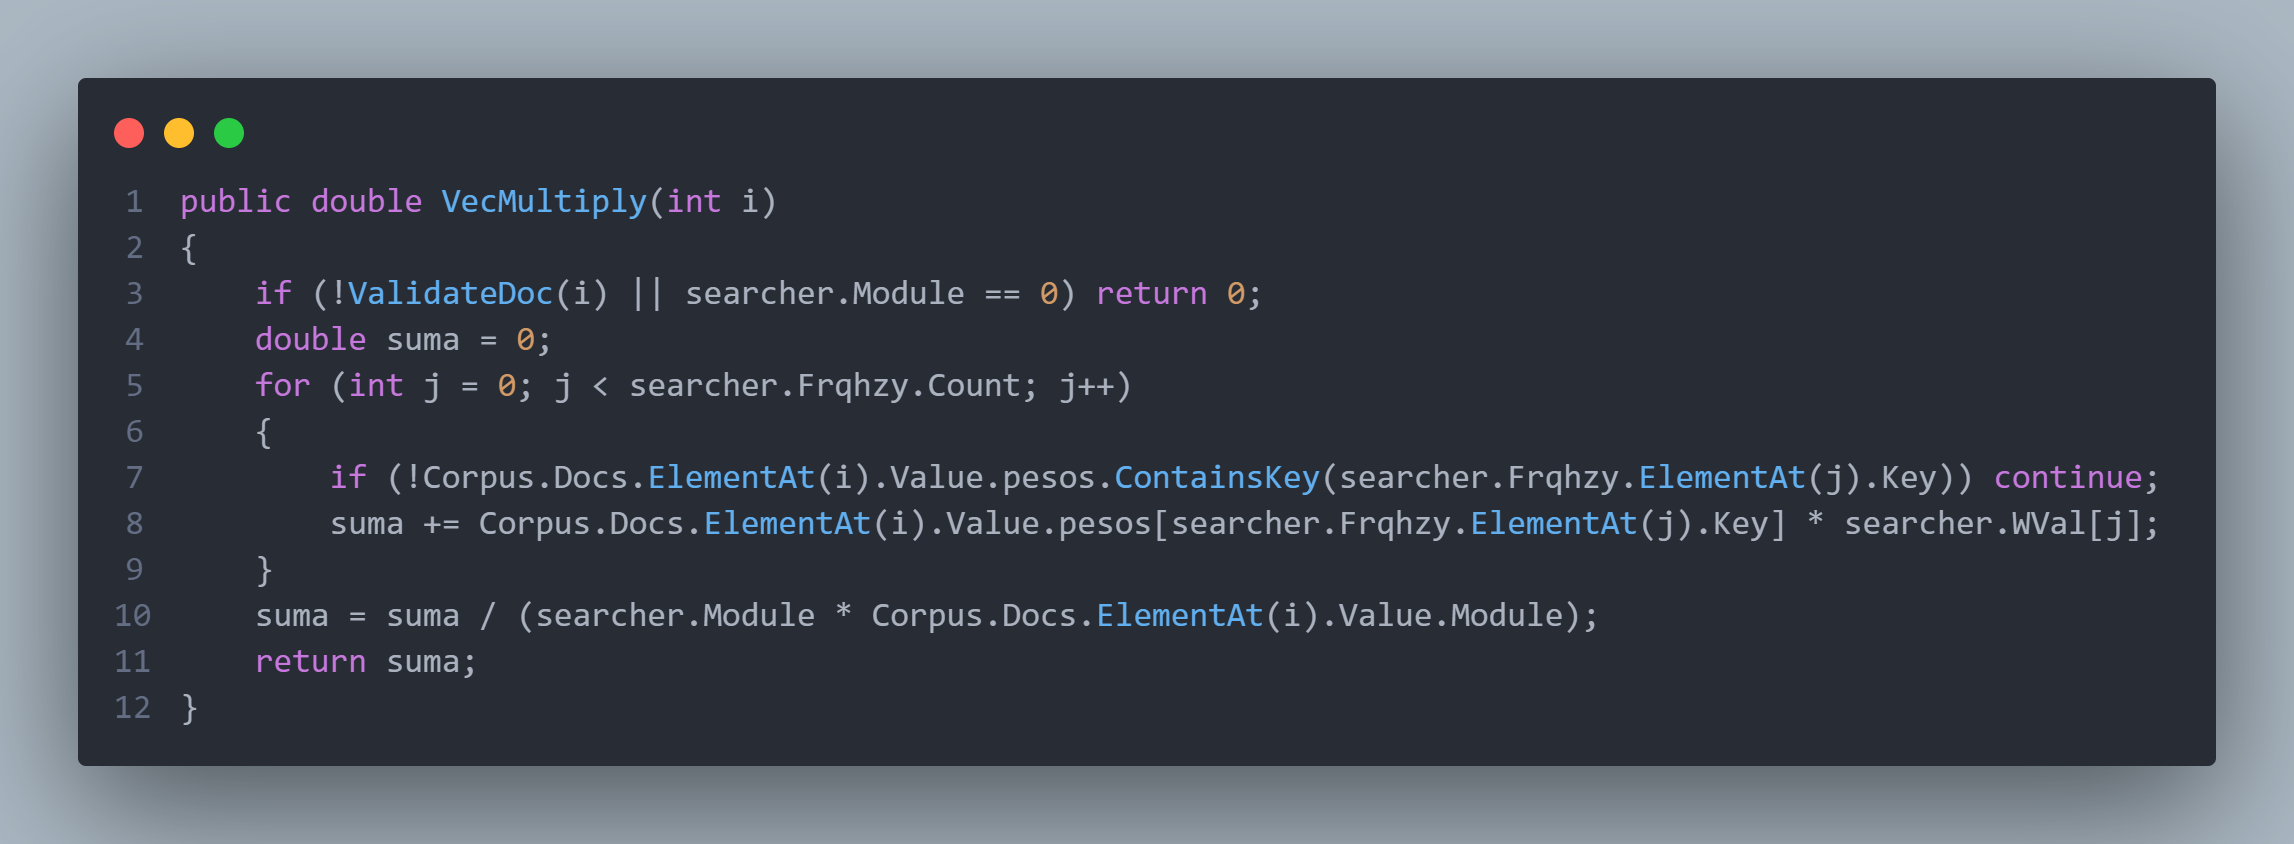
\includegraphics[width=250px]{Assets/vec_mult.png}
        \caption{Poco algebraico no?}
    \end{figure}
\end{frame}

\subsection*{Snippet}
\begin{frame}
    \centering
    
\includegraphics[width=150px]{Assets/snippet_logo.png}
\end{frame}

\begin{frame}
    \begin{abstract}
        Un snippet o fragmento de código, es esa pequeña parte reusable que muestro debajo del título de cada documento, una vez la consulto haya finalizado.
        \begin{figure}
            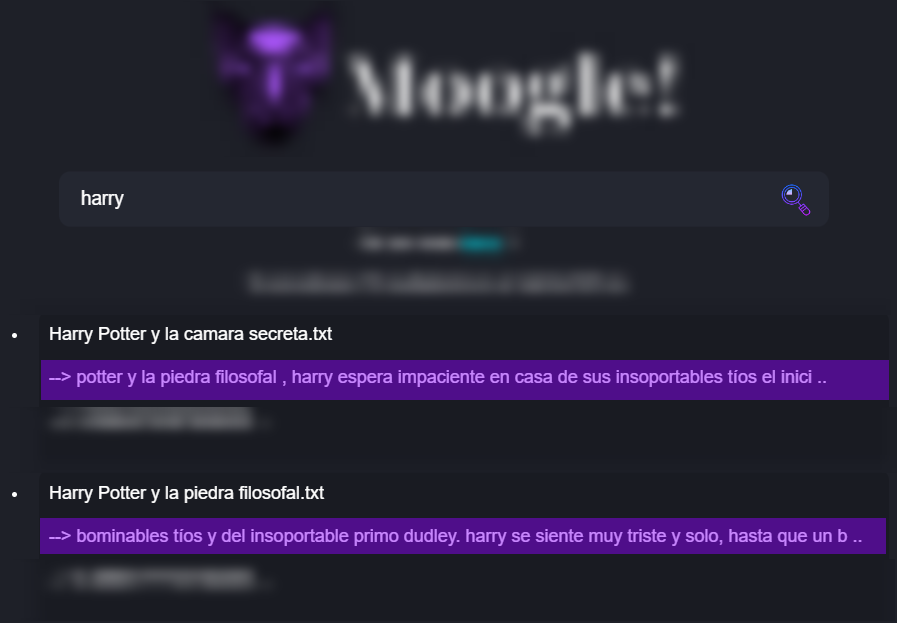
\includegraphics[width=200px]{Assets/snippet_show.png}
        \end{figure}
    \end{abstract}
\end{frame}

\begin{frame}
    La funcion \fbox{FillSnippet()} es la que se encargará de generar y devolver cada snippet presente en aquellos documentos que hayan pasado la consulta.
    \begin{figure}
        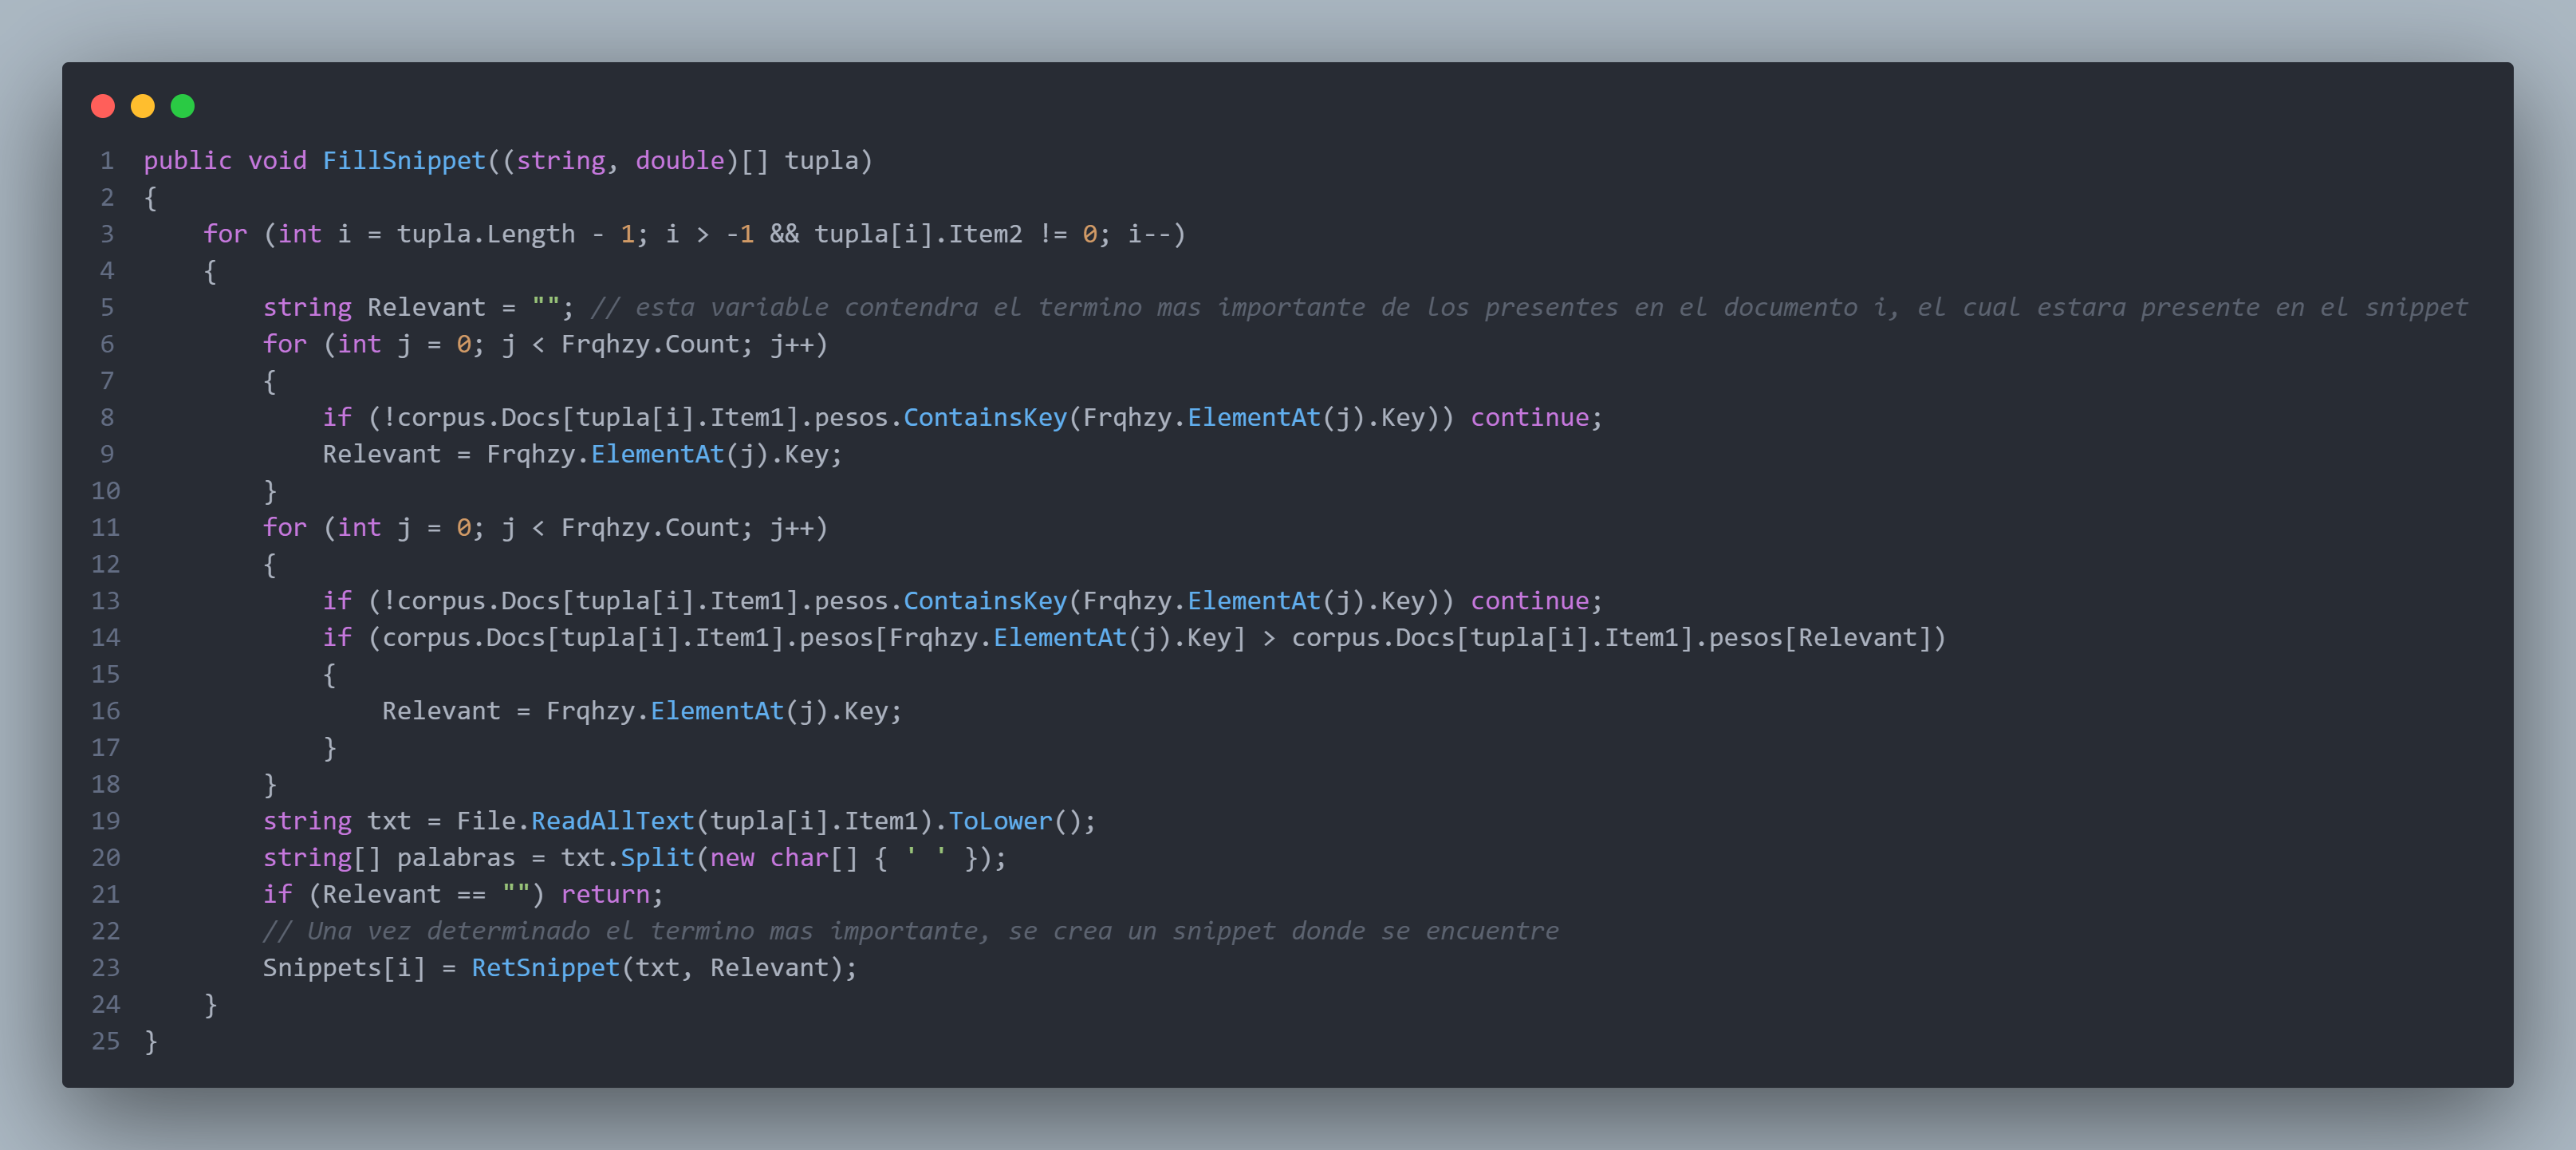
\includegraphics[width=270px]{Assets/fill_snippet.png}
    \end{figure}
    Como se puede observar arriba, es una función bastante grande, donde cada función realizada dentro esta explicada también en el Informe. Además destacar que esta función se invoca en el sorteo de burbuja, mientras se van organizando lso textos a mostrar.
\end{frame}